\section{Параллелограммы и трапеции}

\subsection*{Параллелограммы}

{

\begin{wrapfigure}{r}{40mm}
\vskip-7mm
\centering
\includegraphics{mppics/ris-96}
\caption{}\label{1938/ris-96}
\end{wrapfigure}

\paragraph{Параллелограмм.}\label{1938/87}
Четырёхугольник, у которого противоположные стороны попарно параллельны, называется \rindex{параллелограмм}параллелограммом.
Такой четырёхугольник ($ABCD$, рис. \ref{1938/ris-96}) получится, например, если какие-нибудь две параллельные прямые $KL$ и $MN$ пересечём двумя другими параллельными прямыми $RS$ и $PQ$.

}

\paragraph{}\label{1938/88}
\mbox{\so{Теорема}} (выражающая свойство сторон и углов параллелограмма).
\textbf{\emph{Во всяком параллелограмме противоположные стороны равны, противоположные углы равны и сумма углов, прилежащих к одной стороне, равна $\bm{180\degree}$}} (рис.~\ref{1938/ris-97}).

\begin{wrapfigure}{o}{35mm}
\centering
\includegraphics{mppics/ris-97}
\caption{}\label{1938/ris-97}
\end{wrapfigure}

Проведя диагональ $BD$, мы получим два треугольника:
$ABD$ и $BCD$, которые равны, потому что у них $BD$ — общая сторона, $\angle 1 \z= \angle 4$ и $\angle 2 = \angle 3$ (как накрест лежащие при параллельных прямых).
Из равенства треугольников следует:
$AB=CD$, $AD=BC$ и $\angle A \z= \angle C$.
Противоположные углы $B$ и $D$ также равны, так как они представляют собой суммы равных углов.

Наконец, углы, прилежащие к одной стороне, например углы $A$ и $B$, дают в сумме $180\degree$, так как это углы внутренние односторонние при параллельных прямых.

{\small
\smallskip
\so{Замечание}.
Равенство противоположных сторон параллелограмма иногда кратко выражают другими словами, так:
\emph{отрезки параллельных, отсекаемые параллельными, равны.}

}

{

\begin{wrapfigure}{r}{41mm}
\centering
\vskip-6mm
\includegraphics{mppics/ris-98}
\caption{}\label{1938/ris-98}
\end{wrapfigure}

\smallskip
\mbox{\so{Следствие}.}
\emph{Если две прямые параллельны, то все точки каждой из них одинаково удалены от другой параллельной;
короче:
параллельные прямые \emph{($AB$ и $CD$ рис.~\ref{1938/ris-98})} везде одинаково удалены одна от другой.}

Действительно, если из каких-нибудь двух точек $M$ и $N$ прямой $CB$ опустим на $AB$ перпендикуляры $MP$ и $NQ$, то эти перпендикуляры параллельны (§~\ref{1938/71}), и потому фигура $MNQP$ — параллелограмм;
отсюда следует, что $MP=NQ$, то есть точки $M$ и $N$ одинаково удалены от прямой~$AB$.

}

\paragraph{Два признака параллелограммов.}\label{1938/89}\ 

\smallskip
\mbox{\so{Теорема}.}
\textbf{\emph{Если в выпуклом четырёхугольнике:}}

1) \textbf{\emph{противоположные стороны равны между собой или}}

2) \textbf{\emph{две противоположные стороны равны и параллельны, то такой четырёхугольник есть параллелограмм.}}
Пусть фигура $ABCD$ (рис.~\ref{1938/ris-99}) есть четырёхугольник, у которого.
\[AB=CD\quad \text{и}\quad BC=AB.\]
Требуется доказать, что эта фигура — параллелограмм, то есть что $AB\parallel CD$ и $BC \parallel AD$.
Проведя диагональ $BD$, мы получим два треугольника, которые равны, так как у них $BD$ — общая сторона, $AB\z=CD$ и $BC = AD$ (по условию).
Из равенства этих треугольников следует:
$\angle 1 = \angle 4 $ и $\angle 2 = \angle 3$ (в равных треугольниках против равных сторон лежат равные углы);
вследствие этого $AB \parallel CD$ и $BC\parallel AD$ (если накрест лежащие углы равны, то прямые параллельны).

\begin{wrapfigure}{o}{36mm}
\centering
\includegraphics{mppics/ris-99}
\caption{}\label{1938/ris-99}
\end{wrapfigure}

2) Пусть в четырёхугольнике ($ABCD$, рис.~\ref{1938/ris-99}) $BC\parallel AD$ и $BC = AD$.
Требуется доказать, что $ABCD$ есть параллелограмм, то есть что $AB \parallel CD$.

Треугольники $ABD$ и $BCD$ равны, потому что у них $BD$ — общая сторона, $BC = AD$ (по условию) и $\angle 2 = \angle 3$ (как накрест лежащие углы при параллельных прямых).
Из равенства треугольников следует:
$\angle 1 = \angle 4$;
поэтому $AB\parallel CD$.

\paragraph{}\label{1938/90}
\so{Теорема} (выражающая свойство диагоналей параллелограмма).
\textbf{\emph{Если четырёхугольник}} ($ABCD$, рис.~\ref{1938/ris-100}) \textbf{\emph{— параллелограмм, то его диагонали, пересекаясь, делятся пополам.}}

{

\begin{wrapfigure}[9]{r}{44mm}
\vskip-4mm
\centering
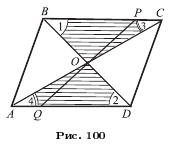
\includegraphics{mppics/ris-100}
\caption{}\label{1938/ris-100}
\end{wrapfigure}

Обратно:
\textbf{\emph{если в четырёхугольнике диагонали точкой их пересечения делятся пополам, то данный четырёхугольник — параллелограмм.}}

1) Треугольники $BOC$ и $AOD$ равны, потому что у них:
$BC\z=AD$ (как противоположные стороны параллелограмма), $\angle 1 = \angle 2$ и $\angle 3 = \angle 4$ (как накрест лежащие при параллельных прямых).

Из равенства треугольников следует:
$OC=OA$ и $OB=OD$.


2) Если $AO=OC$ и $BO=OD$, то треугольники $AOD$ и $BOC$ равны (по двум сторонам и углу между ними).
Из равенства треугольников следует:
$\angle 1 = \angle 2$ и $\angle 3 = \angle 4$.
Следовательно, $BC \parallel AD$ (углы накрест лежащие равны) и $BC=AD$;
поэтому фигура $ABCD$ есть параллелограмм.

}

\paragraph{Центр симметрии.}\label{1938/91}
\textbf{\emph{Параллелограмм, имеет центр симметрии}}, причём центром симметрии служит точка пересечения диагоналей (рис.~\ref{1938/ris-100}).

Действительно, так как $BO=OD$ и $OC=OA$, то отрезки $BC$ и $AD$ симметричны относительно точки $O$ и каждой точке $P$ отрезка $BC$ соответствует симметричная ей точка $Q$ отрезка $AB$ (§~\ref{1938/85}).
Таким же образом убеждаемся, что отрезки $AB$ и $CD$ симметричны относительно той же точки $O$.
Если параллелограмм повернуть вокруг точки пересечения его диагоналей на $180\degree$, то новое положение параллелограмма совпадёт с первоначальным.
При этом каждая из его вершин поменяется местом с противоположной вершиной 
(на рис.~\ref{1938/ris-100} вершина $A$ с $C$ и $B$ с $D$).

\subsection*{Прямоугольник, ромб и квадрат}

\paragraph{Прямоугольник и его свойства.}\label{1938/92}
Если один из углов параллелограмма прямой, то три остальных его угла также прямые (§~\ref{1938/88}).
Параллелограмм, у которого все углы прямые, называется \rindex{прямоугольник}\textbf{прямоугольником}.

Так как прямоугольник есть параллелограмм, то он обладает всеми свойствами параллелограмма;
например, диагонали его делятся пополам и точка их пересечения есть центр симметрии.
Но у прямоугольника есть ещё свои особые свойства.

1) \emph{В прямоугольнике \emph{($ABCD$, рис.~\ref{1938/ris-101})} диагонали равны.}

Прямоугольные треугольники $ACD$ и $ABD$ равны, потому что у них:
$AD$ — общий катет и $AB=CD$ (как противоположные стороны параллелограмма).
Из равенства треугольников следует:
$AC = BD$.

2) \emph{Прямоугольник имеет две оси симметрии.}
Именно, каждая прямая, проходящая через центр симметрии прямоугольника и параллельная двум его противоположным сторонам, есть ось его симметрии.
Эти оси симметрии перпендикулярны между собой (смотри рис. \ref{1938/ris-102}).

\begin{figure}[h]
\begin{minipage}{.32\textwidth}
\centering
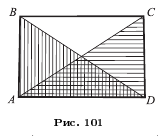
\includegraphics{mppics/ris-101}
\end{minipage}\hfill
\begin{minipage}{.32\textwidth}
\centering
\includegraphics{mppics/ris-102}
\end{minipage}\hfill
\begin{minipage}{.32\textwidth}
\centering
\includegraphics{mppics/ris-103}
\end{minipage}

\medskip

\begin{minipage}{.32\textwidth}
\centering
\caption{}\label{1938/ris-101}
\end{minipage}\hfill
\begin{minipage}{.32\textwidth}
\centering
\caption{}\label{1938/ris-102}
\end{minipage}\hfill
\begin{minipage}{.32\textwidth}
\centering
\caption{}\label{1938/ris-103}
\end{minipage}
\vskip-4mm
\end{figure} 

\paragraph{Ромб и его свойства.}\label{1938/93}
Параллелограмм, у которого все стороны равны, называется \rindex{ромб}ромбом.
Конечно, ему принадлежат все свойства параллелограмма, но у него есть следующие два особых свойства.

1) \emph{Диагонали ромба \emph{($ABCD$, рис.~\ref{1938/ris-103})} взаимно перпендикулярны и делят углы ромба пополам.}
Треугольники $ABD$ и $BDC$ равны, потому что у них:
$BD$ — общая сторона, $AB=BC$ (так как у ромба все стороны равны) и $AO=OC$ (так как диагонали всякого параллелограмма делятся пополам).
Из равенства треугольников следует:
\[\angle 1 =\angle 2,
\quad
\text{то есть}
\quad
BD\perp AC
\quad
\text{и}
\quad
\angle 3 =\angle 4,
\]

\begin{wrapfigure}[20]{o}{34mm}
\vskip-6mm
\centering
\includegraphics{mppics/ris-104}
\captionof{figure}{}\label{1938/ris-104}
\bigskip
\includegraphics{mppics/ris-105}
\caption{}\label{1938/ris-105}
\end{wrapfigure}

\noindent
то есть угол $B$ делится диагональю пополам.
Из равенства треугольников $BOC$ и $COD$ заключаем, что угол $C$ делится диагональю пополам.

2) \emph{Каждая диагональ ромба есть его ось симметрии.}


Диагональ $BD$ (рис.~\ref{1938/ris-104}) является осью симметрии ромба $ABCD$,
то есть вращая $\triangle ABD$ вокруг $BD$, мы можем совместить его с $\triangle BCD$.
В самом деле, диагональ $BD$ делит углы $B$ и $D$ пополам и, кроме того, $AB=BC$ и $AD=CD$.

То же самое можно сказать о диагонали $AC$.

\paragraph{Квадрат и его свойства.}\label{1938/94}\rindex{квадрат}
Квадратом называется параллелограмм, у которого все стороны равны и все углы прямые;
можно также сказать, что квадрат — это прямоугольник, у которого стороны равны, или ромб, у которого углы прямые.
Поэтому квадрату принадлежат все свойства параллелограмма, прямоугольника и ромба.
Например, у квадрата имеется четыре оси симметрии (рис.~\ref{1938/ris-105}):
две, проходящие через середины противоположных сторон (как у прямоугольника), и две, проходящие через вершины противоположных углов (как у ромба).

\subsection*{Теоремы, основанные на свойствах параллелограмма}

\paragraph{}\label{1938/95}
\so{Теорема}.
\textbf{\emph{Если на одной стороне угла}} (например, на стороне $BC$ угла $ABC$, рис.~\ref{1938/ris-106}) \textbf{\emph{отложим равные между собой отрезки}} ($DE=EF=\dots$) \textbf{\emph{и через их концы проведём параллельные прямые}} ($DM$, $EN$, $FP,\dots$) \textbf{\emph{до пересечения с другой стороной угла, то и на этой стороне отложатся равные между собой отрезки}} ($MN=NP=\dots$).
Проведём вспомогательные прямые $DK$ и $EL$, параллельные $AB$.
Полученные при этом треугольники $DKE$ и $ELF$ равны, так как у них:
$DE=EF$ (по условию), $\angle KDE=\angle LEF$ и $\angle KED = \angle LFE$ (как углы, соответственные при параллельных прямых).
Из равенства этих треугольников следует:
$DK=EL$.
Но $DK\z=MN$ и $EL\z=NP$ (как противоположные стороны параллелограммов);
значит, $MN=NP$.

\begin{figure}[!ht]
\centering
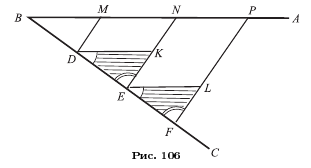
\includegraphics{mppics/ris-106}
\caption{}\label{1938/ris-106}
\end{figure}

{\small
\smallskip
\mbox{\so{Замечание}.}
Равные отрезки могут быть откладываемы и от вершины угла $B$, то есть
так:
$BD=DE= EF=\dots$.
Тогда и на другой стороне равные отрезки надо считать от вершины угла, то есть так:
$BM=MN=NP=\dots$.

}

\paragraph{}\label{1938/96}
\mbox{\so{Следствие}.}
\emph{Прямая \emph{($DE$, рис.~\ref{1938/ris-107}),} проведённая через середину стороны ($AB$) треугольника параллельно другой его стороне ($AC$), делит третью сторону ($BC$) пополам.}

\begin{wrapfigure}[8]{r}{30mm}
\vskip-4mm
\centering
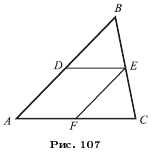
\includegraphics{mppics/ris-107}
\caption{}\label{1938/ris-107}
\end{wrapfigure}


Действительно, мы видим, что на стороне угла $B$ отложены равные отрезки $BD=DA$ и через точки деления $D$ и $A$ проведены параллельные прямые $DE$ и $AC$ до пересечения со стороной $BC$;
значит, по доказанному, на этой стороне тоже отложатся равные отрезки $BE=EC$, и потому $BC$ разделится в точке $E$ пополам.

{\small
\smallskip
\mbox{\so{Замечание}.}
Отрезок, соединяющий середины двух сторон треугольника, называется его \rindex{средняя линия!треугольника}\textbf{средней линией}.

}

\paragraph{}\label{1938/97}
\so{Теорема} (о средней линии треугольника).
\textbf{\emph{Прямая}} ($DE$, рис.~\ref{1938/ris-107}), \textbf{\emph{проведённая через середины двух сторон треугольника, параллельна третьей его стороне;
отрезок этой прямой, лежащий внутри треугольника, равен половине третьей стороны.}}

Для доказательства вообразим, что через середину $D$ стороны $AB$ мы провели прямую, параллельную стороне $AC$.
Тогда, по доказанному в предыдущем параграфе, эта прямая разделит сторону $BC$ пополам и, следовательно, сольётся с прямой $DE$, соединяющей середины сторон $AB$ и $BC$.

Проведя ещё $EF \parallel AD$, найдём, что сторона $AC$ также разделится пополам в точке $F$;
значит, $AF=FC$ и, кроме того, $AF=DE$
(как противоположные стороны параллелограмма $ADEF$), откуда следует:
\[DE=\tfrac12AC.\]

\renewcommand{\bottomtitlespace}{.11\textheight}%определяет минимальную часть текста внизу страницы после заголовка

\subsection*{Трапеции}

\begin{wrapfigure}{r}{40mm}
\vskip-6mm
\centering
\includegraphics{mppics/ris-ru-108}
\caption{}\label{1938/ris-108}
\end{wrapfigure}

\paragraph{}\label{1938/98}
Четырёхугольник, у которого две противоположные стороны параллельны, а две другие не параллельны, называется \rindex{трапеция}\textbf{трапецией}.
Параллельные стороны трапеции ($AD$ и $BC$) называются \rindex{основание!трапеции}\textbf{её основаниями}, непараллельные ($AB$ и $CD$) — \rindex{боковая сторона трапеции}\textbf{боковыми сторонами} (рис.~\ref{1938/ris-108}).
Если боковые стороны равны, трапеция называется \rindex{равнобочная трапеция}\textbf{равнобочной}.

\paragraph{Средняя линия трапеции.}\label{1938/99}
Прямая, соединяющая середины боковых сторон трапеции, называется \rindex{средняя линия!трапеции}\textbf{её средней линией}.
Линия эта обладает следующим свойством.

\smallskip
\mbox{\so{Теорема}.}
\textbf{\emph{Средняя линия}} ($EF$, рис.~\ref{1938/ris-109}) \textbf{\emph{трапеции параллельна основаниям, и равна их полусумме.}}

Через точки $B$ и $F$ проведём прямую до пересечения с продолжением стороны $AD$ в некоторой точке $G$.
Тогда получим два треугольника:
$BCF$ и $DFG$, которые равны, так как у них:
$CF=FD$ (по условию), $\angle BFC\z=\angle DFG$ (как углы вертикальные) и $\angle BCF \z= \angle FDG$ (как углы накрест лежащие при параллельных прямых).
Из равенства треугольников следует:
$BF=FG$ и $BC=DG$.
То есть в треугольнике $ABG$ прямая $EF$ соединяет середины двух сторон, значит (§~\ref{1938/97}), $EF \parallel AG$ и $EF = \tfrac12(AD+DG)$, другими словами, $EF\parallel AD$ и $EF \z= \tfrac12(AD + BC)$.

\begin{figure}[h]
\begin{minipage}{.54\textwidth}
\centering
\includegraphics{mppics/ris-109}
\end{minipage}\hfill
\begin{minipage}{.44\textwidth}
\centering
\includegraphics{mppics/ris-110}
\end{minipage}

\medskip

\begin{minipage}{.54\textwidth}
\centering
\caption{}\label{1938/ris-109}
\end{minipage}\hfill
\begin{minipage}{.44\textwidth}
\centering
\caption{}\label{1938/ris-110}
\end{minipage}
\vskip-4mm
\end{figure} 

\paragraph{}\label{1938/100}
\mbox{\so{Задача}.}
\emph{Данный отрезок \emph{($AB$, рис.~\ref{1938/ris-110})} разделить на данное число равных частей} (например, на~3).

Из конца $A$ проводим прямую $AC$, образующую с $AB$ какой-нибудь угол;
откладываем на $AC$ от точки $A$ три произвольной величины и равных между собой отрезка:
$AD$, $DE$ и $EF$;
точку $F$ соединяем с $B$;
наконец, из $E$ и $D$ проводим прямые $EN$ и $DM$, параллельные $FB$.
Тогда отрезок $AB$, по доказанному, разделится в точках $M$ и $N$ на три равные части.

{\small

\subsection*{Задачи на построение}


\paragraph{Метод параллельного перенесения.}\label{1938/101}
На свойствах параллелограмма основан особый приём решения задач на построение, известный под названием метода параллельного перенесения.
Его сущность лучше всего выяснить на примере.

\begin{wrapfigure}{r}{45mm}
\vskip-7mm
\centering
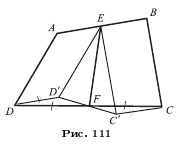
\includegraphics{mppics/ris-111}
\caption{}\label{1938/ris-111}
\end{wrapfigure}

\smallskip
\mbox{\so{Задача}.}
Построить четырёхугольник $ABCD$ (рис.~\ref{1938/ris-111}), зная все его стороны и отрезок $EF$, соединяющий середины противоположных сторон.

Чтобы сблизить между собой данные линии, перенесём параллельно самим себе стороны $AD$ и $BC$ в положения $ED'$ и $EC'$.
Тогда сторона $DD'$ будет равна и параллельна $AE$, а сторона $CC'$ равна и параллельна $BE$, но так как $AE=BE$, то $DD'=CC'$ и $DD'\parallel CC'$.
Вследствие этого треугольники $DD'F$ и $CC'F$ будут равны (так как у них:
$DD' = CC'$, $DF=FC$ и $\angle D'DF=\angle FCC'$), значит, $\angle D'FD=\angle C'FC$ и потому линия $D'FC'$ должна быть прямая, то есть
фигура $ED'FC'$ окажется треугольником.
В этом треугольнике известны две стороны ($ED'=AD$ и $EC'=BC$) и медиана $EF$, проведённая к третьей стороне.
По этим данным легко построить треугольник $ED'C'$ (если на продолжении медианы $EF$ за точку $E$ отложим отрезок, равный $EF$, и полученную точку соединим с $D'$ и $C'$, то получим параллелограмм, у которого известны стороны и одна диагональ).

Найдя $\triangle ED'C'$, строим затем треугольники $D'DF$ и $C'CF$, а затем и весь четырёхугольник $ABCD$.

Предоставляем самим учащимся с помощью этого метода решить следующие задачи:

\medskip

1.
Построить трапецию по одному её углу, двум диагоналям и средней линии.

2.
Построить четырёхугольник по трём сторонам $a$, $b$, $c$ и двум углам $\alpha$ и $\beta$, прилежащим к неизвестной стороне.

3.
Построить трапецию по четырём данным её сторонам.

\paragraph{Метод симметрии.}\label{1938/102}
Свойства осевой симметрии также могут быть использованы при решении задач на построение.
Иногда искомый приём построения легко обнаруживается, если перегнём часть чертежа вокруг некоторой прямой так, чтобы эта часть заняла симметричное положение по другую сторону от этой прямой.
Приведём пример:

\smallskip
\so{Задача}.
\emph{На прямой $AB$ \emph{(рис.~\ref{1938/ris-112})} найти точку $x$, чтобы сумма расстояний от $x$ до данных точек $M$ и $N$ была наименьшая.}

\begin{wrapfigure}{o}{40mm}
\vskip-0mm
\centering
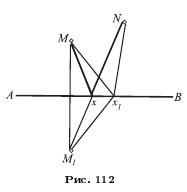
\includegraphics{mppics/ris-112}
\caption{}\label{1938/ris-112}
\end{wrapfigure}

Если, перегнув чертёж вокруг $AB$, приведём точку $M$ в симметричное относительно $AB$ положение $M'$, то расстояние от точки $M$ до какой угодно точки прямой $AB$ равно расстоянию от точки $M'$ до той же точки прямой $AB$.
Поэтому суммы $Mx\z+xN,  Mx_1\z+x_1N,\dots $ равны соответственно суммам $M'x+xN, M'x_1\z+x_1N, \dots$;
но из последних сумм наименьшая будет та, при которой линия $M'xN$ — прямая.
Отсюда становится ясным приём построения.

То же самое построение решает и другую задачу:
\emph{на прямой $AB$ найти такую точку $x$, чтобы прямые $xM$ и $xN$, проведённые от неё к данным точкам $M$ и $N$, составляли с $AB$ равные углы.}

Предоставляем учащимся решить методом симметрии следующие задачи:

\medskip

1.
Построить по четырём сторонам четырёхугольник $ABCD$, зная, что его диагональ $AC$ делит угол о пополам.

2.
На прямоугольном бильярде дано положение двух шаров $A$ и $B$.
В каком направлении надо толкнуть шар $A$, чтобы он, отразившись последовательно от всех четырёх бортов, ударил затем шар $B$.

3.
Дан угол и внутри него точка.
Построить треугольник наименьшего периметра, такой, чтобы одна его вершина лежала в данной точке, а две другие на сторонах угла.

}

{\small

\subsection*{Упражнения}


\begin{center}
\so{Доказать теоремы}
\end{center}

\begin{enumerate}[noitemsep]

\item
Соединив последовательно середины сторон какого-нибудь четырёхугольника, получим параллелограмм.

\item
В прямоугольном треугольнике медиана, проведённая к гипотенузе, равна её половине.

\smallskip
\so{Указание}.
Следует продолжить медиану на расстояние, равное её длине.

\item
Обратно:
если медиана равна половине стороны, к которой она проведена, то треугольник прямоугольный.

\item
В прямоугольном треугольнике медиана и высота, приведённые к гипотенузе, образуют угол, равный разности острых углов треугольника.

\smallskip
\so{Указание}.
См.
задачу 2.

\item
В $\triangle ABC$ биссектриса угла $A$ встречает сторону $BC$ в точке $D$;
прямая, проведённая из $D$ параллельно $CA$, встречает $AB$ в точке $E$;
прямая, проведённая из $E$ параллельно $BC$, встречает $AC$ в $F$.
Доказать, что $EA=FC$.

\item
Внутри данного угла построен другой угол, стороны которого параллельны сторонам данного и равно отстоят от них.
Доказать, что биссектриса построенного угла лежит на биссектрисе данного угла.

\item
Всякая прямая, соединяющая какую-нибудь точку нижнего основания трапеции с какой-нибудь точкой верхнего основания, делится средней линией пополам.

\item
В треугольнике через точку пересечения биссектрис углов, прилежащих к основанию, проведена прямая параллельно основанию.
Доказать, что отрезок, заключённый между боковыми сторонами треугольника, равен сумме отрезков боковых сторон, считая их от основания.

\item
Через вершины углов треугольника проведены прямые, параллельные противоположным сторонам.
Доказать, что образованный ими треугольник составлен из четырёх треугольников, равных данному, и что каждая сторона его в два раза более соответствующей стороны данного треугольника.

\item
В равнобедренном треугольнике сумма расстояний от каждой точки основания до боковых сторон есть величина постоянная, а именно:
она равна высоте, опущенной на боковую сторону.

\item
Как изменится эта теорема, если взять точку на продолжении основания.

\item
В равностороннем треугольнике сумма расстояний всякой точки, взятой внутри этого треугольника, до сторон его есть величина постоянная, равная высоте треугольника.

\item
Всякий параллелограмм, у которого диагонали равны, есть прямоугольник.

\item
Всякий параллелограмм, у которого диагонали взаимно перпендикулярны, есть ромб.

\item
Всякий параллелограмм, у которого диагональ делит угол пополам, есть ромб.

\item
Из точки пересечения диагоналей ромба опущены перпендикуляры на стороны ромба.
Доказать, что основания этих перпендикуляров образуют вершины прямоугольника.

\smallskip
\so{Указание}.
См.
задачу 13.

\item
Биссектрисы углов прямоугольника своим пересечением образуют квадрат.

\item
Пусть $A'$, $B'$, $C'$ и $B'$ будут середины сторон $CD$, $DA$, $AB$ и $BC$ квадрата.
Доказать, что отрезки $AA'$, $CC'$, $BB'$ и $DD'$ образуют своим пересечением квадрат, сторона которого равна $\tfrac25$ каждого из этих отрезков.

\item
Дан квадрат $ABCD$.
На сторонах его отложены равные части $AA_1$, $BB_1$, $CC_1$ и $DD_1$.
Точки $A_1$, $B_1$, $C_1$, $D_1$ соединены последовательно прямыми.
Доказать, что $A_1B_1C_1D_1$ есть квадрат.

\item
Если середины сторон какого угодно четырёхугольника взять за вершины нового четырёхугольника, то последний есть параллелограмм.
Определить, при каких условиях этот параллелограмм будет:
1) прямоугольником, 2) ромбом, 3) квадратом.

\end{enumerate}

\begin{center}
\so{Найти геометрические места}
\end{center}

\begin{enumerate}[noitemsep]


\item
Середин всех отрезков, проведённых из данной точки к различным точкам данной прямой.

\item
Точек, равно отстоящих от двух параллельных прямых.

\item
Вершины треугольников, имеющих общее основание и равные высоты.
\end{enumerate}
\begin{center}
\so{Задачи на построение}
\end{center}

\begin{enumerate}[resume,noitemsep]

\item
Даны два угла треугольника;
построить третий.

\item
Дан острый угол прямоугольного треугольника;
построить другой острый угол.

\item
Провести прямую, параллельную данной прямой и находящуюся от неё на данном расстоянии.

\item
Разделить пополам угол, вершина которого не помещается на чертеже.

\item
Через данную точку провести прямую под данным углом к данной прямой.

\item
Даны две прямые $XY$ и $X'Y'$ и точка $F$;
провести через эту точку такую секущую, чтобы часть её, заключённая между данными прямыми, делилась точкой $F$ пополам.

\item
Через данную точку провести прямую так, чтобы отрезок её, заключённый между двумя данными параллельными прямыми, равнялся данному отрезку.

\item
Между сторонами данного острого угла поместить отрезок данной длины так, чтобы он был перпендикулярен к одной стороне угла.

\item
Между сторонами данного угла поместить отрезок данной длины параллельно заданной прямой, пересекающей обе стороны данного угла.

\item
Между сторонами данного угла поместить отрезок данной длины так, чтобы он отсекал от сторон угла равные отрезки.

\item
Построить прямоугольный треугольник по данным:
острому углу и противолежащему катету.

\item
Построить треугольник по двум углам и стороне, лежащей против одного из них.

\item
Построить \so{равнобедренный} треугольник по углу при вершине и основанию.

\item
То же — по углу при основании и высоте, опущенной на боковую сторону.

\item
То же — по боковой стороне и высоте, опущенной на неё.

\item
Построить равносторонний треугольник по его высоте.

\item
Разделить прямой угол на три равные части (другими словами, построить угол, равный  $30\degree$).

\item
Построить треугольник по основанию, высоте и боковой стороне.

\item
То же — по основанию, высоте и углу при основании.

\item
То же — по углу и двум высотам, опущенным из стороны этого угла.

\item
То же — по стороне, сумме двух других сторон и высоте, опущенной на одну из этих сторон.

\item
То же — по высоте, периметру и углу при основании.

\item
Провести в треугольнике прямую, параллельную основанию, так, чтобы отрезок, заключённый между боковыми сторонами, был равен сумме отрезков боковых сторон, считая от основания.

\item
Построить многоугольник, равный данному.

\smallskip
\so{Указание}.
Диагоналями разбивают данный многоугольник на треугольники.

\item
Построить \so{четырёхугольник} по трём его углам и двум сторонам, образующим четвёртый угол.

\smallskip
\so{Указание}.
Надо найти четвёртый угол.

\item
То же — по трём сторонам и двум диагоналям.

\item
Построить \so{параллелограмм} по двум неравным сторонам и одной диагонали.

\item
То же — по стороне и двум диагоналям.

\item
То же — по двум диагоналям и углу между ними.

\item
То же — по основанию, высоте и диагонали.

\item
Построить \so{прямоугольник} по диагонали и углу между диагоналями.

\item
Построить \so{ромб} по стороне и диагонали.

\item
То же — по двум диагоналям.

\item
То же — по высоте и диагонали.

\item
То же — по углу и диагонали, проходящей через этот угол.

\item
То же — по диагонали и противолежащему углу.

\item
То же — по сумме диагоналей и углу, образованному диагональю со стороной.

\item
Построить \so{квадрат} по данной диагонали.

\item
Построить \so{трапецию} по основанию, прилежащему к нему углу и двум непараллельным сторонам (могут быть два решения, одно и ни одного).

\item
То же — по разности оснований, двум боковым сторонам и одной диагонали.

\item
То же — по четырём сторонам (всегда ли задача имеет решение?).

\item
То же — по основанию, высоте и двум диагоналям (условие существования решения).

\item
То же — по двум основаниям и двум диагоналям (условие существования решения).

\item
Построить \so{квадрат} по сумме стороны с диагональю.

\item
То же — по разности диагонали и стороны.

\item
Построить \so{параллелограмм} по двум диагоналям и высоте.

\item
То же — по стороне, сумме диагоналей и углу между ними.

\item
Построить треугольник по двум сторонам и медиане, проведённой к третьей стороне.

\item
То же — по основанию, высоте и медиане, проведённой к боковой стороне.

\item
Построить \so{прямоугольный треугольник} по гипотенузе и сумме катетов (исследовать).

\item
То же — по гипотенузе и разности катетов.

\item
Даны две точки $A$ и $B$, расположенные по одну сторону от данной прямой $XY$.
Расположить на этой прямой отрезок $MN$ данной длины $\ell$ так, чтобы ломаная $AM+MN+NB$ была наименьшей длины.

\smallskip
\so{Указание}.
Приблизим точку $B$ к точке $A$, двигая её по прямой, параллельной $XY$, на расстояние, равное $MN$.

\end{enumerate}

}
